\documentclass[a4paper]{scrartcl}     % scrartcl

\usepackage{fullpage}
\usepackage{natbib}            % Use Natbib style for the refs.
\usepackage{booktabs}
\usepackage{pdflscape}
\usepackage[headsep=0.8cm]{geometry}
\usepackage{longtable}
\usepackage{tabu}
\usepackage{multicol}
\usepackage{enumitem}
\usepackage{graphicx}
\usepackage{caption}
\usepackage{subcaption}
\usepackage{setspace}
\usepackage[hyphens]{url}
\usepackage[english]{babel}
\usepackage[utf8]{inputenc}
\newcommand{\ignore}[1]{}


\usepackage{enumitem}
\setlist[description]{leftmargin=\parindent,labelindent=\parindent}

\usepackage{fancyhdr}
\pagestyle{fancy}

%%% METADATA
\usepackage[pdftex,pdfborderstyle={/S/U/W 0}]{hyperref}
\makeatletter
\AtBeginDocument{
  \hypersetup{
    pdftitle = {\@title},
    pdfauthor = {\@author}
  }
}
\makeatother

\setfootnoterule[0.4pt]{\textwidth}% default height is 0.4pt

\setlength{\parindent}{0cm} % Default is 15pt
\setlength{\parskip}{0.3cm plus4mm minus3mm}

\newif\ifbreaksection

\breaksectiontrue

%\raggedbottom

\title{The Dangers of Patient Data in Clinical Decision Making}
\author{Peter West}

\begin{document}

\begin{titlepage}
  \makeatletter
  \begin{center}
    {\LARGE University of Southampton}\\[0.5cm]
    {\Large Web Science CDT}\\[3.0cm]
    %{\huge \bfseries Using Personal Informatics to Support Decision-Making in Healthcare: A Survey of the Dangers of Cognitive Bias} \\ [1.0cm]
    \begin{spacing}{2}
      {\huge \bfseries \@title} \\ [1.0cm]
    \end{spacing}
    {\Large by
       \@author \\[1.0cm]}
    {\Large
      Supervisors:\\[0.2cm]
      Dr. Richard Giordano\\[0.1cm]
      Dr. Max Van Kleek \\[0.7cm]
      Examiner:\\[0.2cm]
      Dr. David Millard\\[3.5cm]
    }
    {\Large \today}
    \vfill
    {\Large A dissertation submitted in partial fulfilment of the degree of}\\[0.5cm]
    {\Large MSc Web Science}
  \end{center}
  \makeatother
\end{titlepage}

\thispagestyle{empty}
\null\vspace{\fill}
\begin{center}
  {\large \textsf{\textbf{Abstract}}}
\end{center}
\begin{abstract}
  The increasing ubiquity of personal tracking devices is leading to the possibility of using health and wellbeing data to support clinical decisions. Hundreds of devices, mobile apps and social networking websites exist to record personal information related to health, including weight, diet and activity. Such data has been demonstrated as providing self-insight and promoting positive health behaviours, such as maintaining a healthy diet. As such, there has been interest in its use by clinicians to support decision making. However, clinicians' ability to interpret data may be prone to cognitive bias and poor judgement.

  Through reviewing literature on the use of personal data and making clinical decisions within time and resource constraints, this dissertation synthesises a series of cognitive biases pertaining to a number of clinical scenarios. From this, the dangers and consequences of their use in healthcare are assessed. In agreement with previous research, the biases identified pose a greater risk within scenarios where there is limited time and resources. Drawing from these results, this dissertation forms framework for future research into data use in clinical scenarios.

  %data sources were first classified using the Roper-Logan-Tierney Model of Living, a prevalent model of nursing within the United Kingdom. In order to survey these risks, scenarios of data use are considered against the biases which may affect them.
\end{abstract}
\vspace{\fill}

\clearpage\thispagestyle{empty}\tableofcontents

\clearpage\section{Acknowledgements}

  Thanks to my supervisors, Dr. Richard Giordano and Dr. Max Van Kleek, for their guidance throughout this project and ongoing discussions on the future of this research. Thanks to Dr. James Wilson for consulting with me about the design of studies in Healthcare. Thanks also to Dr. Jeff Vass for his ongoing contributions to this research.


\clearpage\section{Introduction} % 100%

  % background (set the stage)
  The explosion of social networking websites, mobile apps and consumer devices for tracking personal information has created many new detailed data sources about health and wellbeing. This information has been demonstrated to promote positive health behaviours, such as encouraging a healthy diet \citep{Brown2006}, assisting in recovery of cancer patients \citep{Jacobs2014}, and reminding people to take their medication \citep{Stawarz2014}. These benefits have led calls to investigate the use of consumer technology within health care \citep{Swan2009}. It has been proposed that such personal information can form a body of patient data to support clinical decision making, in turn leading to more accurate diagnoses, improved patient outcomes, and reduced mortality \citep{Rooksby2014}.

  % problem
  Recent research has revealed that clinical decision making is often negatively affected by cognitive bias, leading to preventable adverse events, worsened patient outcomes, and higher mortality \citep{Croskerry2013}. \citet{Graber2002} states that cognitive bias is a major cause of preventable diagnostic error, but is extremely challenging to study and reduce. This complements earlier discoveries by \citet{Kahneman1982}, in which people tend to use biases when making decisions under uncertainty, occasionally leading to severe errors. Many forms of cognitive bias have been identified -- Wikipedia lists over 350\footnote{Wikipedia -- List of cognitive biases -- \url{http://en.wikipedia.org/wiki/List_of_cognitive_biases} [Accessed 4th Sep 2014]} -- however, the consequences of biases in clinical decision making remain largely unexplored \citep{Croskerry2013}. It is thus unknown how the provision of patient data may affect bias in clinical decisions.

  % research questions
  By conducting a literature review of research in cognitive bias over the last 50 years, this dissertation presents a list of 11 cognitive biases which may affect clinical decisions made when patient data is used. From this, it has been identified that supplementing patient data may introduce further bias due to methods clinicians use to interpret patient data. Furthermore, it has been found that these biases usually have a more significant effect when decisions are made in acute scenarios, such as emergency rooms, where decisions must be made quickly with limited resources.

  % definitions
  For the purpose of this dissertation, decisions which involve patient data are called \textit{evidence-based clinical decisions}. The term \textit{patient data} refers specifically to personal information which is collected by mobile apps and consumer devices, such as the number of steps taken, video lifelogs, location history and status updates on social networks. Patient data is subsequently \textit{interpreted} by clinicians, which refers to the observation, analysis and sense-making of data.

  % motivation
  The purpose of this literature review is threefold. First, in identifying biases which affect clinical decision making, this research raises consciousness to the effect of bias in evidence-based clinical decisions. In turn, it is hoped that clinicians' increased understanding of bias may help reduce the frequency of adverse events, improve patient outcomes and reduce mortality. Second, in identifying the cases where biases are of high risk, this research proposes a number of steps which may be taken by data scientists and health scientists to avoid bias in evidence-based clinical decisions. Third, current research is limited in the area of bias in clinical decisions, and the effect of providing patient data has not yet been investigated. This research provides a framework for conducting such investigations by proposing a number of hypotheses formed from the identified biases.

  % methodology
  The literature review was conducted in five stages. The first stage comprised of identifying cognitive biases that affect clinical decision making. This largely builds on previous research by Patrick Croskerry M.D., Ph D. (Division of Medical Education, Dalhousie University). The second stage comprised of identifying cognitive biases which affect data interpretation. This research involved searching in the Cognitive Science journals, and extracts from the books \textit{Nudge: Improving Decisions About Health, Wealth and Happiness} \citep{Thaler2012}, \textit{Thinking, Fast and Slow} \citep{Kahneman2012} and \textit{Predictably Irrational: The Hidden Forces that Shape Our Decisions} \citep{Ariely2009}. The third stage involved synthesising a list of biases which are the product of combining clinical decision making biases and interpretation biases. The fourth stage involved identifying how these biases are affected by restricting time and resources. This involved searching literature for empirical studies of the biases. Finally, stage five involved the categorising of biases by their risk factors and causes.

  % Research contributions
  The disciplines involved in this research include Health Science, Cognitive Science and Computer Science. Each discipline has its own methodological and epistemological approaches, which limits how research from multiple disciplines can by synthesised \citep{Repko2011}. Therefore, this dissertation does not attempt to take a standpoint from any one discipline, and instead opts for an interdisciplinary perspective. The Web Science perspective is particularly useful in this case, as it concerns itself with the study of the World Wide Web within disciplines other than Computer Science. \citet{Hendler2008} states that ``despite the Web's great success as a technology and the significant amount of computing infrastructure on which it is built, it remains, as an entity, surprisingly unstudied.''  It is hoped that the approach and findings in this dissertation will contribute to the growing field of Web Science.


  In concluding, it is argued that the findings from the literature review can be used to raise consciousness to the effect of biases in evidence-based clinical decision making. Suggestions are made for the design of patient data in order to minimise these biases. Finally, a framework for future empirical studies within clinical scenarios is proposed. It is hoped that the findings from these studies will inform research of bias leading to better understanding of their nature and consequences.

  % Signpost
  This dissertation first discusses the background material, detailing research relating to health data, technology in clinical environments and decision economics. Following an overview of related work, three research questions are distilled and their importance underlined. The methodology for conducting the literature review is then described. The results are stated, followed by a discussion of the causes and effects of biases in clinical environments. This dissertation concludes by forming a framework for future research.


\ifbreaksection\clearpage\fi\section{Background} % 100%

  This section overviews the background in three areas. First, the use of health and wellbeing data in industry, personalised medicine and healthcare is considered. Second, the barriers to the acceptance of technology in healthcare are examined. Finally, the field of decision economics is reviewed, focusing on the effects of bias and environment.

  \subsection{Health and Wellbeing Data}\label{sec:background:data}

    % from intro
    % This information has been demonstrated to promote positive health behaviours, such as encouraging a healthy diet , assisting in recovery of cancer patients , and reminding people to take their medication . These benefits have led calls to investigate the use of consumer technology within health care \citep{Swan2009}. It has been proposed that such personal information can form a body of patient data to support clinical decision making, in turn leading to more accurate diagnoses, improved patient outcomes, and reduced mortality \citep{Rooksby2014}.

    The increasing usage of sophisticated mobile devices is leading to a greater number of people recording data about their daily life. \citet{Swan2009} has studied the use of this data as a means to supplement healthcare, which would increase ``information flow, transparency, customization, collaboration and patient choice and responsibility taking, as well as quantitative, predictive and preventive aspects.'' There has been support from the Personalised Medicine community to use personal data in improving personal health \citep{Li2011}. Industry is also pushing for more health tracking devices, apps and social networks \citep{U.S.FoodandDrugAdministration2014}. These three parties -- industry, Personalised Medicine and healthcare -- are intricately linked in the design of tools to be used by patients and clinicians \citep{Taneva2014}. These are discussed below.

    \subsubsection{Industry}

      %industry
      Within industry, a number social networking websites, consumer devices and mobile apps have come to market which enable the collection of lifestyle data. These products take various forms, including wearable products, ambient technologies, websites, and APIs. Among these are the Nike+ Fuelband\footnote{Nike+ Fuelband -- \url{http://www.nike.com/us/en_us/c/nikeplus-fuelband} [Accessed 4th Sep 2014]} (a wrist-worn activity tracker), Facebook\footnote{Facebook -- \url{http://www.facebook.com} [Accessed 4th Sep 2014]} (a social networking website which allows status updates), the Jawbone Up\footnote{Jawbone Up -- \url{https://jawbone.com/up} [Accessed 4th Sep 2014]} (a wrist-worn sleep tracker) and Moves\footnote{Moves App -- \url{https://www.moves-app.com/} [Accessed 4th Sep 2014]} (a mobile app for tracking activity). An extensive list of over 500 such products is available on the Quantified Self community website\footnote{Quantified Self Guide -- \url{http://quantifiedself.com/guide/} [Accessed 4th Sep 2014]}.  The Quantified Self Guide categorises these products by the type of data they collect, offering the following categories (with the number of products in parentheses): energy (36), fitness (124), food (54), goals (87), health (185), learning (20), lifelogging (122), lifestyle (76), location (57), medicine (60), money (33), mood (59), productivity (55), relationships (19), sleep (34), and social (95).

      %Industry in healthcare
      More recently, large manufacturers have been proposing healthcare applications for their products, including Apple\footnote{MobiHealthNews: Apple reveals tracking app HealthKit and partners with Mayo Clinic, Epic -- \url{http://mobihealthnews.com/33728/apple-reveals-tracking-app-healthkit-and-partners-with-mayo-clinic-epic/} [Accessed 4th Sep 2014]}, Google\footnote{MobiHealthNews: Google unveils Google Fit, a fitness platform for developers -- \url{http://mobihealthnews.com/34430/google-unveils-google-fit-a-fitness-platform-for-developers/} [Accessed 4th Sep 2014]} and Samsung\footnote{MobiHealthNews: Samsung unveils prototype health device a week before Apple’s expected Healthbook launch -- \url{http://mobihealthnews.com/33595/samsung-unveils-prototype-health-device-a-week-before-apples-expected-healthbook-launch/} [Accessed 4th Sep 2014]}, indicating that there will likely be imminent growth of the sector. There also appears to be an increasing awareness of the application of technology to health. The U.S. Food and Drug Administration has recently approved the use of two wrist-worn fitness trackers for clinical trials, citing the importance of quantifiable analysis of physical activity to physiological monitoring \citep{U.S.FoodandDrugAdministration2014}.

    \subsubsection{Personalised Medicine}

      % communities
      The growth of industry surrounding lifestyle data has led to the creation and shift of a number of communities:
      \begin{description}
        \item[Quantified Self] is an emerging community which focuses on the use of technology to record everyday activities, such as the number of steps walked or how well one eats \citep{Choe2014}. On the motivations behind Quantified Self, \citet{Choe2014} found that people want to track their activity primarily to help improve their health. Other reasons include maximising work performance, and finding new life experiences.

        \item[Personal Informatics] is a new field dedicated to understanding the individual collection of personal data. \citet{Li2010} defines Personal Informatics as ``systems as those that help people collect personally relevant information for the purpose of self-reflection and gaining self-knowledge.'' This field is particularly concerned with the human nature of personal data \citep{Rooksby2014}, and to how data is made accessible via visualisations and mashups \citep{Bentley2013}.

        \item[Ubiquitous Computing] is a field of computing which studies the use of computers `everywhere'. This field has seen recent growth due to the emergence of mobile devices capable to recording personal information. Ubiquitous computing concerns include the design of mobile platforms \citep{Gurrin2013}, what data may be used for \citep{Li2011}, and how data may be visualised \citep{Lee2014}.

        \item[Lifelogging] is the act of automatically recording everyday lifestyle activities \citep{Doherty2011}. Like ubiquitous computer, this area has grown due to the increasing pervasiveness of technology. For example, Microsoft SenseCam is a small camera which has been demonstrated to help in dieting, market analysis and as a memory prosthetic \citep{Doherty2011,Doherty2013}.
      \end{description}

      % personalised medicine
      These communities have gained attention in the field of Personalised Medicine, which deals with medical treatment of people based on their individual biological characteristics \citep{Swan2009}. In particular, \citet{Swan2012} argues for a patient-centric approach to healthcare by way of personalised recommendations delivered from health and wellbeing data. The pervasive nature of personal devices allows tracking of minor lifestyle activities which would otherwise not be noteworthy \citep{Rooksby2014}. These previously-unavailable details may be extremely useful to the diagnosis and care \citep{Swan2012}.

      %self-reflection
      In support of its usefulness, a number of studies have demonstrated the use of health and wellbeing data to encourage self-reflection and improved health. \citet{Bentley2013} demonstrated that allowing people to link various health and wellbeing data together allowed people to reflect and change their behaviours. For example, when mood, food and weather were visualised together, subjects we able to gain insight into the causes of bad moods thus encouraging behaviour changes to avoid those situations. Subjects also found that they walked less on particular days of the week, are happier when are less tired, and slept better when exercised more. \citet{Cuttone2014} demonstrated a number of visualisations which were effective for self-reflection on quantified self data. Self-reflection is also documented by \citep{Kamal2010}, who review literature on social networks to argue that social pressure also encourages self reflection. These demonstrations of self-reflection have encouraged the design of numerous personal health apps, including dieting \citep{Choe2014}, cancer recovery \citep{Jacobs2014}, and medication taking \citep{Stawarz2014,Lee2014}.

      %model
      %\citep{Li2010} has formalised a stage-based model to describe, in which people prepare for data collection, undergo data collection, integrate the data with other tools, reflect on it and take action. Further to this, \citep{Li2011} find that people need visualisations

    \subsubsection{Healthcare}

      \citet{Swan2009} has called for use of this data as a means to supplement healthcare, which would increase ``information flow, transparency, customization, collaboration and patient choice and responsibility taking, as well as quantitative, predictive and preventive aspects.''. The use of self-tracking data in healthcare is not new. The health diary has been popular since the 1950's as a data collection method \citep{Richardson1994}.  \citet{Richardson1994} note that particular types of data that are recorded include pain, fatigue, medication use and dietary intake. This shares overlap with health and wellbeing data, suggesting there are existing use cases where health and wellbeing data could be supplemented. \citet{OLoughlin2013} has demonstrated the use of lifelogging for the purpose of increasing diet awareness. However, \citet{Swan2009} has discussed that there is currently little adoption, perhaps due to the barriers of technology in clinical environments.

  \subsection{Technology in Clinical Environments}

    % from intro

    %use of technology in healthcare

    The use of technology within Healthcare is necessarily highly restrictive. Previous technology failures in clinical environments have led to incorrect diagnoses, malfunctions and patient deaths \citep{Leveson1993}. One particular case is that of Therac-25, a radiation therapy machine, which, due to oversights and mistakes in software development, management and quality control, massively overdosed six people between 1985 and 1987 \citep{Leveson1993}. Restrictions on technology therefore raise the barrier for technology adoption. \citet{Boonstra2010} identifies eight categories of barriers of electronic health records: financial, technical, time, psychological, social, legal, organizational, and change process.

    \citet{Beuscart-Zephir1997}, \citet{Ovretveit2007} and \citet{Taneva2014} propose design considerations for effective implementation technology. Their hope is that by raising awareness of the issues of clinical environments raised by \citet{Boonstra2010}, developers will take a critical approach, leading to greater technology acceptance. One success case is the recent acceptance of telemedicine \citep{Chau2002}. There has been some interest by clinicians for greater technology adoption. \citet{Croskerry2013a} states the decision support systems should be encouraged as a way to reduce error. However, Croskerry concedes that clinicians are resistant, as it takes time and effort to load information into decisions support systems and undermines their own knowledge.



    %design of technology in healthcare

    %Assessing the usability of technology in healthcare . . Design in healthcare .

    %models of technology in healthcare

    %As such, models of using technology in healthcare have become prevelent. One particular model is Evidence-based healthcare \citep{Heneghan2013}. Mobile patient monitoring \citep{Wac2009}. Patient driven healthcare model \citep{Swan2009}, Personalised medicine \citep{Swan2012}. Health diary \citep{Richardson1994}. As described, cameras more accurate than written diary \citep{OLoughlin2013}.

    % decision support
    % - decision support - don't get used (should be) - incumberant - load information into system... resent because it takes a long time to load information + physicians think they know already + financial. Inertia against it. Doctors miss things on differential diagnosis. Relevant information put into decision support system by someone else so that physicians don't need to (using clinical time) ----- head towards this - all appropriate information provided = better support ``medical watson'' - clinician still crucial for interpretation of information that comes out.


    %co-care

  \subsection{Decision Making}\label{sec:background:biases}

    There is extensive literature surrounding the psychology of decision making. Below, literature from three topics in are discussed: cognitive bias, systems of thought and thin-slice and resource-rich scenarios.

    \subsubsection{Cognitive Bias}\label{sec:background:biases:cog}


      % thinking fast and slow - thinking models, negative effects
      Humans are prone to errors in decision making. Over the last four decades, a number of researchers have attempted to categorise and study the reasons for errors. In particular, cognitive bias is a well accepted model which can explain human error. \citet{Kahneman2012} provides an extensive overview of the empirical research into cognitive bias in decision making. Bias is a lack of reasoning in making a decision, leading to systematic error in decision making and violating the rules of rational choice. \citet{Thaler2012} concur with this, stating that humans make mistakes due to heuristics and fallacies. \citet{Graber2002} state that despite the inevitability of human error, cognitive errors may be reduced by system level changes, including second opinions and decision-support systems. % Specific biases can be overcome - debiasing \citep{Kahneman1982}, but bias in overcoming bias \citet{Croskerry2003}.

      % nudge -

      % - humans don't think "unfailingly well" - make mistakes due to heuristics and fallacies
      % - building on kahneman2012
      % - libertarian paternalist (influence people to make better choices)



      % predictably irrational
      %\citet{Ariely2009}

      %many biases - 351 on wikipedia, Sackett (1979) 56 biases on academic research alone

      % Biases affecting judgement:
      % - Anchoring
      % - Availability
      % - Representativeness


      %  Specific biases can be overcome - debiasing \citep{Kahneman1982}, but bias in overcoming bias \citet{Croskerry2003}


    %Recent research has revealed that clinical decision making is often negatively affected by cognitive bias, leading to preventable adverse events, worsened patient outcomes, and higher mortality \citep{Croskerry2013}. \citet{Graber2002} states that cognitive bias is a major cause of preventable diagnostic error, but is extremely challenging to study and reduce. This complements earlier discoveries by \citet{Kahneman1982}, in which people tend to use biases when making decisions under uncertainty, occasionally leading to severe errors. Many forms of cognitive bias have been identified -- Wikipedia lists over 350\footnote{Wikipedia -- List of cognitive biases \url{http://en.wikipedia.org/wiki/List_of_cognitive_biases} [Accessed 4th Sep 2014]} -- however, the consequences of biases in clinical decision making remain largely unexplored \citep{Croskerry2013}. It is thus unknown how the provision of patient data may affect bias in clinical decisions.

    \subsubsection{Systems of Thought}

      In an attempt to understand the situations in which biases occur, \citet{Kahneman2012} describe two systems that are used when making a decision: Automatic and Reflective. \citet{Thaler2012} suggest that the Automatic system is used in decisions which are made rapidly and intuitively, while the Reflective system is used when decisions need to be made more consciously and deliberately.  \citet{Kahneman2012} state that uncertainty leads to use of the Automatic system. \citeauthor{Thaler2012} list a number of characteristics and examples of these systems, as shown in Table~\ref{table:thaler}.


      \begin{table}[htb]
        \caption{Characteristics of the automatic and reflective systems with example problems which might invoke those systems \citep{Thaler2012}.}
        \renewcommand{\arraystretch}{1.5}
        \begin{tabu}{X[0.6,l] X[2,p] X[2,p]}
        \toprule
        System & Characteristics & Examples \\
        \midrule
        Automatic
          & gut reaction, intuitive, uncontrolled, effortless, associative, fast, unconscious, skilled
          & Ducking when a ball is thrown at you; Getting nervous in airplanes during turbulence; Smiling at the sight of a cute puppy. \\

        Reflective
          & conscious thought, rational, controlled, effortful, deductive, slow, self-aware, rule-following
          & When asked `How must is 411 times 37?'; Deciding a route between two points on a map; Choosing a discipline to study. \\
        \bottomrule
        \end{tabu}
        \label{table:thaler}
      \end{table}



      % objective vs intuition
      %Objective decision making \citep{Mellor1983}. Intuition - the good and the bad. Prolonged practice leads to the accurate intuition of experts.



    \subsubsection{Thin-Slice and resource-rich Environments}\label{sec:background:biases:scenarios}

      Research on cognitive bias has revealed that biases are invoked depending on the environment. Environments where time and resources are constrained lead to increased use of bias \citep{Kahneman2012}. Further, environments where decisions must be made quickly with preference for the Automatics system are common in clinical scenarios. Nurses in emergency rooms, for example, must make decisions rapidly, often using intuition \citep{Cioffi1997}. \citet{Croskerry2005} refers to this as Flesh and Blood decision making:
      \begin{quote}
        ``Flesh and Blood decisionmaking, occurs when `the cognitive reality departs from the formalized ideal.' James Reason used the expression to describe what often happens in the course of practical decisionmaking. Clinicians do not take to reclining armchairs to cogitate and consider their options at length, but instead respond to omnipresent time pressures and resource availability with expeditious decision and action. To make a Flesh and Blood decision is to think on one's feet and go with clinical intuition. Those who can make good Flesh and Blood decisions use health care resources sparingly.''  \citep{Croskerry2005}
      \end{quote}

      \noindent Scenarios in which resources are so tightly constrained will, for the purpose of this dissertation, be called \textit{thin-slice scenarios}. In contrast, \citet{Croskerry2005} describes the more resourceful Formal Work-up:

      \begin{quote}
       ``In the Formal Work-Up, both the hypothesis context and acuity are clearer. The patient may `look sick' or there may be features of the presentation that mandate a search for significant or serious illness. The first response from the clinician may require an active intervention to stabilize the patient, but there follows a formal investigation with iterative hypothesis testing and refinement toward a definitive diagnosis. The overall decision by the physician regarding which of the three decision modes to use ultimately reflects the quality of calibration. For expedient and safe care, the right decision style must be matched to the appropriate clinical situation.''  \citep{Croskerry2005}
      \end{quote}

      \noindent Scenarios in which there is plentiful time and resources, with preference for the Reflective System, will be called \textit{resource-rich}. Table~\ref{table:clinscenarios} lists a number of characteristics and examples of these scenarios.

      %overview
      %Literature in cognitive bias has shown evidence of increased occurrence in %situations of uncertainty or when time and resources are constrained.

      %thin-slice
      %Thin-slice = acute scenario (Croskerry) = automatic . Thin slicing leads to greater use of biases and heuristics (sad --> affect \citep{Ambady2002})

      %resource-rich
      %Resource-rich = Reflective \citep{Kahneman2012}

      %

       \begin{table}[htb]
        \caption{Clinical Scenarios}
        \renewcommand{\arraystretch}{1.5}
        \begin{tabu}{X[1,l] X[2,p] X[2,p]}
        \toprule
        Scenario & Characteristics & Examples \\
        \midrule
        Thin-slice
          & time constraints, limited resources, quick decisions, automatic thinking, acute scenario, Flesh and Blood, little access to information and little clinical patient history
          & emergency room, patient room, general practice \\
        Resource-rich
          & slow decisions, reflective thinking, formal workup, deliberative, access to supplementary information and extensive clinician-patient history
          & general practice, careers, physiotherapist \\
        \bottomrule
        \end{tabu}
        \label{table:clinscenarios}
      \end{table}

\ifbreaksection\clearpage\fi\section{Related Work}\label{sec:related} % 100%

  This section gives an overview of related work in clinical decision making. This mostly draws from the research of Patrick Croskerry M.D., Ph D. (Division of Medical Education, Dalhousie University), who has provided insight into how cognitive biases affect clinical decisions, but also considers research into cognitive biases and case studies in Health Science.

  \citet{Croskerry2003} states that current theorists in clinical decision making are resistant to move on from normative models, which model decision making as rational and objective.  These models have no real practical application as they do not consider the time, resource and financial constraints that typically occur in clinical environments \citep{Croskerry2003}. As discussed in Section~\ref{sec:background:biases}, these constraints are ideal conditions for bias, errors and ultimately failed patients \citep{Kahneman2012}. More problematic still, \citet{Croskerry2003a} proposes that biases are covert and subtle, making them more difficult to observe and making clinicians unaware of them, which, Croskerry suggests, is perhaps why they are not on the list of serious reportable events\footnote{List of Serious Reportable Events -- \url{http://www.qualityforum.org/Topics/SREs/List_of_SREs.aspx} [Accessed 4th Sep 2014]}.

  There has only recently been empirical studies into the nature of clinical decision biases. A study conducted at a Utah hospital found highest percentage of negligent adverse events occurred in patient rooms and emergency rooms \citep{Thomas2000}. \citeauthor{Thomas2000} suggest task complexity, uncertainty, multiple concurrent tasks, changing plans and high workload may be factors in this. Further, in a Australia hospital study by \citet{Wilson1995}, 51\% of adverse events were judged to have high preventability. In particular, averse events resulting from decision making errors generally associated with high preventability. This research suggests a need to identify causes of decision making errors in order to reduce adverse events.

  In an attempt to classify decision making errors, \citet{Croskerry2002} lists 30 biases and heuristics that affect clinical decision making, collectively known as \textit{Cognitive Dispositions to Respond} (CDRs). These are particularly prevalent in thin-slice conditions, such as emergency rooms. These biases are listed in Table~\ref{table:cdrs}. For each, \citeauthor{Croskerry2002} describes its effect on clinical decision making, both in terms of what may be observed and the potential consequences, and provides a discussion on how they may be avoided, citing existing empirical studies. The CDRs identified by \citet{Croskerry2002} affect all clinical decisions, and are thus of key importance in identifying biases which affect evidence-based clinical decision making.



      \begin{table}
        \caption{30 Cognitive Dispositions to Respond identified by \citet{Croskerry2002}.}
        \renewcommand{\arraystretch}{0}
        \begin{tabu} to \linewidth {X[1,l]}
          \toprule
          \begin{multicols}{3}
           \begin{itemize}[label={}]
            \item Aggregate bias
            \item Anchoring
            \item Ascertainment bias
            \item Availability and non-availability
            \item Base-rate neglect
            \item Commission bias
            \item Confirmation bias
            \item Diagnosis momentum
            \item Fundamental attribution error
            \item Gambler's fallacy
            \item Gender bias
            \item Hindsight bias
            \item Multiple alternatives bias
            \item Omission bias
            \item Order effects
            \item Outcome bias
            \item Overconfidence bias
            \item Playing the odds
            \item Posterior probability error
            \item Premature closure
            \item Psych-out error
            \item Representativeness restraint
            \item Search satisfying
            \item Sutton's slip
            \item Triage-cueing
            \item Unpacking principle
            \item Vertical line failure
            \item Visceral bias
            \item Yin–yang out
            \item Zebra retreat
          \end{itemize}
          \end{multicols} \\
          \bottomrule
        \end{tabu}
        \label{table:cdrs}
      \end{table}

  \citet{Graber2002} have provided some insight into cognitive errors in clinical decisions, in particular pertaining to data collection and interpretation, flawed reasoning and incomplete knowledge. Examples of these errors are listed in Table~\ref{table:graber}. \citet{Graber2002} highlight data interpretation as one area of cognitive error, explaining expertise is a large factor in the ability to reliably interpret data:




  \begin{quote}
  ``The probability of the initial hypothesis is adjusted upwards or downwards using test results to calculate a new probability using Bayes' theorem. Unfortunately, few clinicians are skilled in using Bayes' theorem, and in practice it is probably more common for tests to be interpreted without taking into account the characteristics (sensitivity and specificity) of the test itself.'' \citep{Graber2002}
  \end{quote}

  Research has demonstrated the cognitive effects on data interpretation beyond just expertise. Experiments have demonstrated evidence of the availability heuristic in interpreting graphed data \citep{Spirrison1994}, priming between data sets \citep{Jalal2014}, affect and representativeness heuristics \citep{Peters2006}, the framing effect with varying contexts \citep{Cheng2012}, and the curse of knowledge in audible evidence \citep{Lange2011}. However, there appears to be little research into how biases in interpreting data may affect clinical decision making.


  \begin{table}[htb]
    \caption{Examples of cognitive errors \citep{Graber2002}}
    \renewcommand{\arraystretch}{1.5}
    \begin{tabu}{X[1,l] X[2,p]}
    \toprule
    Error & Example \\
    \midrule
    Inadequate knowledge
      & Wrong diagnosis of ventricular tachycardia on ECG with electrical artefact simulating this arrhythmia \\
    Faulty data gathering
      & Missed diagnosis of breast cancer from failure to perform breast examination \\
    Faulty information processing
      & Failing to perceive the lung nodule on a patient's chest X-ray \\
    Faulty metacognition
      & Wrong diagnosis of degenerative arthritis (no further tests ordered) in a patient with septic arthritis \\
    \bottomrule
    \end{tabu}
    \label{table:graber}
  \end{table}

  The literature suggests that biases in clinical decision making are not well explored. \citet{Croskerry2003} has thus called on clinical decision makers to gain an appreciation of the contribution of cognitive error and the impact of diagnostic error, refute the inevitability of cognitive diagnostic errors, and dismiss the pessimism surrounding approaches for lessening cognitive bias.


  % in informatics
  %Lifelogging with wearable cameras briefly raised prospect of  \citep{Kelly2013}


  %Diagnostic uncertainty mot likely in internal, family and emergency medicine



\ifbreaksection\clearpage\fi\section{Research Questions}\label{sec:qs} % 100%

  This section describes the research questions which will be addressed in this dissertation. This research responds to the calls for further research into clinical decision making identified in Section~\ref{sec:related}. When using patient data, what are the consequences of biases in clinical decision making? Answering this mandates the understanding of individual biases in different environments. For example, what is the effect of the availability heuristic in an emergency department?

  The research questions are threefold:

  \begin{description}
    \item[Q1] \textit{How do biases affect evidence-based clinical decision making?}
    \begin{addmargin}[1.9em]{0em}
      As has been suggested by \citet{Graber2002}, data interpretation may lead to bias in clinical decisions. It is thus expected that using patient data will introduce additional bias in clinical decision making.
    \end{addmargin}
    \item[Q2] \textit{What are the risks of biases in thin-slice scenarios?}
    \begin{addmargin}[1.9em]{0em}
      Section~\ref{sec:background:biases} gave an overview of thin-slice scenarios. Empirical evidence suggests that people rely on biases more when in thin-slice scenarios. It is thus expected that there will be a large effect of biases thin-slice scenarios.
    \end{addmargin}
    \item[Q3] \textit{What are the risks of biases in resource-rich scenarios?}
    \begin{addmargin}[1.9em]{0em}
      In Section~\ref{sec:background:biases}, it was found that when provided with sufficient time and resources, biases are less relied on. It is thus expected that there will be a lesser effect of biases resource-rich scenarios.
    \end{addmargin}
  \end{description}

  The following sections describe the methodology of a literature review to investigate these questions, the results from the literature review and a discussions.


\ifbreaksection\clearpage\fi\section{Methodology} % 100%

  This section describes the methodology used to form an understanding of biases which affect evidence-based clinical decision making. \citet{Fink2005} raised the importance of conducting reviews systematically, such that they can be re-applied by others. This requires that methods of identifying literature are explained and justified \citep{Fink2005}. The methodology thus comprises of a stage-based literature review. Stages 1, 2 and 3 pertain to Q1, which involves identifying biases which affect evidence-based clinical decision making. Stage 4 and 5 pertain to Q2 and Q3 in identifying the effects of bias in thin-slice and resource-rich scenarios.



  % Searching
  % - targeted search (in books?)
  % - search strategy (keywords)
  % Selection
  % - inclusion/exclusion criteria (contexts, outcomes sought)
  % - topics of interest
  % Evaluating evidence
  % - study design classification
  % - quality assessment

  \subsubsection*{Stage 1: Identifying cognitive biases which affect clinical decision making}

    As discussed in Section~\ref{sec:related}, there is little research into the effects of biases in clinical decision-making. However, Patrick Croskerry M.D., PhD. (Division of Medical Education, Dalhousie University) has provided some insight into the area with his literature reviews, published by the Society for Academic Emergency Medicine and the New England Journal of Medicine \citep{Croskerry2002,Croskerry2003,Croskerry2013}. One of these reviews in particular, \citet{Croskerry2002}, identified 30 biases and heuristics which affect clinical decision making, collectively called \textit{Cognitive Dispositions to Respond} (CDRs), listed in Table~\ref{table:cdrs}. Because this dissertation specifically concerns the use of data, only CDRs which have affects due to data were selected. These are listed in Table~\ref{table:ibcdrs}, and are the sole contribution of this stage. These biases affect all clinical decisions, and are thus of key importance in identifying biases which affect evidence-based clinical decision making. Thus, when a clinician must make a decision based on a patients presenting complaints, their decision is also affected by CDRs (see Figure~\ref{fig:clinic}).


    \begin{table}
      \caption{Eleven Cognitive Dispositions to Respond affected by interpretation biases.}
      \renewcommand{\arraystretch}{0}
      \begin{tabu} to \linewidth {X[1,l]}
        \toprule
        \begin{multicols}{3}
         \begin{itemize}[label={}]
          \item Aggregate bias
          \item Anchoring
          \item Ascertainment bias
          \item Availability and non-availability
          \item Base-rate neglect
          \item Confirmation bias
          \item Fundamental attribution error
          \item Order effects
          \item Outcome bias
          \item Posterior probability error
          \item Representativeness restraint
        \end{itemize}
        \end{multicols} \\
        \bottomrule
      \end{tabu}
      \label{table:ibcdrs}
    \end{table}

  \subsubsection*{Stage 2: Identifying cognitive biases which affect data interpretation}

    The identification of data interpretation biases was less simple. While there is an abundance of information about biases which affect data interpretation, its pervasive nature means that the literature is spread over numerous disciplines.  The primary sources chosen were the overview literatures described in Section~\ref{sec:background:biases:cog}: \textit{Nudge: Improving Decisions About Health, Wealth and Happiness} \citep{Thaler2012}, \textit{Thinking, Fast and Slow} \citep{Kahneman2012} and \textit{Predictably Irrational: The Hidden Forces that Shape Our Decisions} \citep{Ariely2009}. These books provided an overview of a number of biases, as well as extensive bibliographies. From these, literature which classed cognitive bias or cognitive error and indicated biases in the presence of data interpretation were selected. Ten interpretation biases were thus identified, as shown in Table~\ref{table:irs}. These biases are important to evidence-based clinical decision making as they affect how evidence is identified within patient data (see Figure~\ref{fig:data}).

    \begin{table}
      \caption{Interpretation biases}
      \renewcommand{\arraystretch}{0}
      \begin{tabu} to \linewidth {X[1,l]}
        \toprule
        %\begin{multicols}{2}
         \begin{itemize}[label={}]
            \item Availability \citep{Tversky1973,Spirrison1994}
            \item Affect heuristic \citep{Zajonc1980,Peters2006}
            \item Ambiguity effect \citep{Ellsberg1961a,Crosby2007}
            \item Illusory patterns \citep{Kahneman1974,Whitson2008}
            \item Priming \citep{Meyer1971} %,Jalal2014
            \item Curse of knowledge \citep{ColinCamerer1989,Lange2011}
            \item Framing effect \citep{Tversky1981,Cheng2012}
            \item Functional fixedness \citep{Adamson1952,Adamson1954}
            \item Observer expectancy effect \citep{Mahoney1977,Graber2002}
            \item Extension neglect \citep{KahnemanDaniel2000,Peters2006}
          \end{itemize} \\
        %\end{multicols}
        \bottomrule
      \end{tabu}
      \label{table:irs}
    \end{table}

    \begin{figure}[htb]
      \centering

      \begin{subfigure}[htb]{0.3\textwidth}
        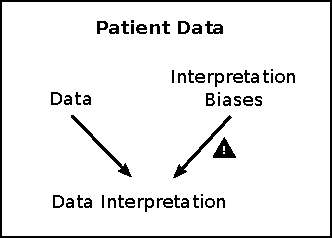
\includegraphics[width=\textwidth]{images/data.pdf}
        \caption{in data interpretation}
        \label{fig:data}
      \end{subfigure}
      ~
      \begin{subfigure}[htb]{0.35\textwidth}
        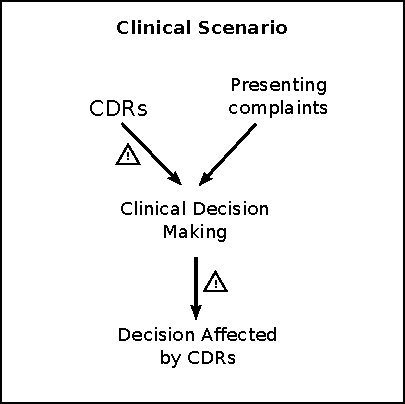
\includegraphics[width=\textwidth]{images/clinic.pdf}
        \caption{in clinical decisions}
        \label{fig:clinic}
      \end{subfigure}

      \caption{Bias effects}\label{fig:effects}
    \end{figure}

  \subsubsection*{Stage 3: Synthesising a list of relevant biases}

    This stage involved synthesising the literature from stages 1 and 2 to form a list of biases which affect evidence-based clinical decision making. In evidence-based clinical decisions, data interpretation must necessarily happen prior to clinical decisions. Therefore, any biases which affect data interpretation (interpretation biases) will affect the decision making process. Figure~\ref{fig:clinicdata} illustrates this, showing that decisions are affected by both interpretation biases and CDRs. This stage thus attempts to form a cohesion between these two forms of bias. For the purpose of this dissertation, the resulting biases from this cohesion are called \textit{Clinical Interpretation Reasoning Biases} (CIRBs).

    \begin{figure}[htb]
      \centering
      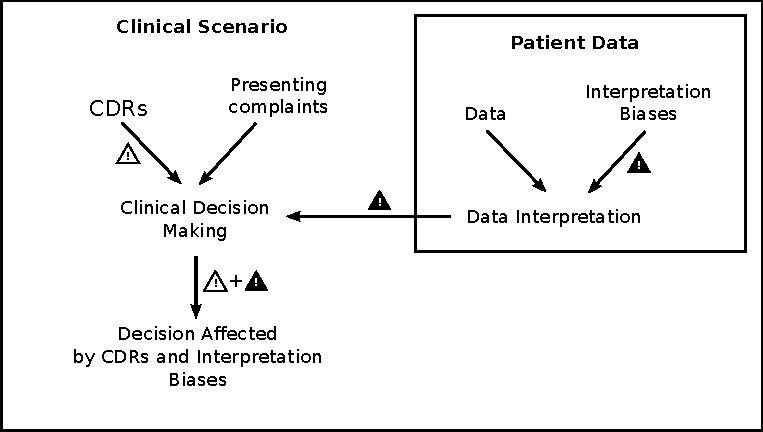
\includegraphics[width=0.7\textwidth]{images/clinic+data.pdf}
      \caption{Bias effects in evidence-based clinical decisions}
      \label{fig:clinicdata}
    \end{figure}


    Mathematically speaking, CIRBs are the union of interpretation biases and CDRs. This is expressed as

    $$ CIRB = IB \cup CDR $$

    \noindent where IB is the set of Interpretive Biases and CDR is the set of Cognitive Dispositions to Respond. Using this, 11 CIRBs were identified, which are listed in Table~\ref{table:cirbs}. Note that those which were deemed sufficiently similar were grouped together.

    \begin{table}
      \caption{Clinical Interpretation Reasoning Biases.}
      \renewcommand{\arraystretch}{0}
      \begin{tabu} to \linewidth {X[1,l]}
        \toprule
        \begin{multicols}{3}
         \begin{itemize}[label={}]
          \item Affect heuristic
          \item Ambiguity effect and Outcome bias
          \item Anchoring and Adjustment
          \item Availability heuristic \columnbreak
          \item Confirmation bias, observer-expectancy effect and ascertainment bias
          \item Curse of knowledge
          \item Framing effect
          \item Functional fixedness
          \item Illusory patterns and Aggregate bias
          \item Priming, Order effects, contrast effect and posterior probability
          \item Representativeness heuristic, extension neglect and base rate neglect
        \end{itemize}
        \end{multicols} \\
        \bottomrule
      \end{tabu}
      \label{table:cirbs}
    \end{table}

  \subsubsection*{Stage 4: Identifying empirical studies}

    This stage involved identifying how CIRBs are affected by restricting time and resources. From Section~\ref{sec:background:biases:scenarios}, two extreme scenarios were selected: thin-slice scenarios, and resource-rich scenarios. Characteristics of these scenarios are listed in Table~\ref{table:clinscenarios}. Identifying empirical studies involved further reading into individual biases, starting with the references listed in stages 1 and 2. In addition a search strategy was used, with terms including ``cognitive bias data analysis'', ``cognitive bias data interpretation'', ``cognitive error data'', ``cognitive limitations data''. As per stage 2, only literature which classed cognitive bias or cognitive error as the primary focus were selected.

    The results of this literature search allowed the forming of a table. For each CIRB, a description is formed from early literature, and its inclusion is justified with regard to why it affects evidence-based clinical decisions. The clinical consequences are also described based on existing literature. Each bias has columns for describing the effects of the bias in thin-slice and resource-rich scenarios. These consist of a  risk summary (high, medium or low risk), and empirical evidence of this risk.

  \subsubsection*{Stage 5: Categorisation by risk factor}

    This stage involved the categorising of CIRBs by their risk factors and causes. This was based on the author's judgement of similarities between biases, including situations in which they show more effect, traits of the clinicians and other external factors.


\ifbreaksection\clearpage\fi\section{Results} % 100%

  This section details the results from the literature synthesis, presented in respect to the research questions stated in Section~\ref{sec:qs}. Drawing from Q1, a table of biases which affect evidence-based clinical decision making is presented. Drawing from Q2 and Q3, the effects of bias in thin-slice scenarios resource-rich scenarios are outlined respectively.

  \subsection{Biases in Evidence-Based Clinical Decision Making}

    Table~\ref{table:cirbs-expanded} lists 11 Clinical Interpretation Reasoning Biases that have been identified, with descriptions and consequences, and risks to thin-slice and resource-rich scenarios. The first column lists CIRBs as identified in Table~\ref{table:cirbs}. The second column provides a description of CIRBs, a justification for their inclusion and an overview of clinical consequences. The third column describes the risk of CIRBs in thin-slice scenarios, describing relevant empirical literature. The fourth column describes the risk of CIRBs in resource-rich scenarios, describing relevant empirical literature. Characteristics and examples of these scenarios are listed in Table~\ref{table:clinscenarios}.

  \subsection{Effects of Bias in Thin-Slice Scenarios}

    A thin-slice scenario is a clinical scenario in which there is heavy time constraints, little access to information and no clinical patient history (see Table~\ref{table:clinscenarios}). It was expected that judgements in thin-slice scenarios are more susceptible to biases. Accordingly, Table~\ref{table:cirbs-expanded} shows that 10 of the identified CIRBs are prevalent in thin-slice scenarios. Among these, it appears that the reasons are fourfold: false pattern recognition, positive tendency, misuse of prior knowledge and poor communication.

    \begin{description}
    \item[False pattern recognition.]
    Biases which are caused by pattern recognition under uncertainty include the representativeness heuristic\ignore{extension neglect, base rate neglect} and illusory patterns\ignore{and aggregate bias}. It has been proposed that, when interpreting data or making decisions under uncertainty, clinicians are more likely to observe pattens which are statistically insignificant \citep{Kahneman1974}, and use these without consideration of the statistical significance \citep{KahnemanDaniel2000}. As has been found by \citet{Bassili2000}, time constraints leads to identification of false patterns. \citet{Tversky1974} and \citet{Bar-Hillel1980} propose that information considered important will outweigh base-rates. Therefore, in uncertainty, clinicians are likely to make decisions based on false patterns over base rates.

    \item[Positive tendency.]
    Biases which are caused by positive tendency under uncertainty include the affect heuristic, the ambiguity effect\ignore{outcome bias} and the framing effect. In thin-slice scenarios, there is a greater dependency on emotion in making decisions, with people more prepared to choose an option if it has favourable outcomes as more competent \citep{Baron1988}. People will choose favourable options based on their probabilities despite not knowing the probabilities of other options \citep{Ellsberg1961a}. Further, people are more likely to choose options when they are phrased positively \citep{Tversky1981}.

    \item[Misuse of prior knowledge.]
    Biases which are caused by misuse of prior knowledge include priming,\ignore{order bias, contrast effect, posterior probability error, anchoring,} the availability heuristic and confirmation bias\ignore{observer-expectancy effect and the ascertainment bias}. These biases affect judgements using: knowledge about previous judgements \citep{Meyer1971,Kahneman1974}; perceived weightings of knowledge \citep{Tversky1973}; or personal beliefs \citep{Mahoney1977}. In cases of constrained time or resources, these biases cause people to use prior knowledge without consideration of its reliability or relevance.

    \item[Poor communication.]
    Only one identified bias relates to poor communication: the curse of knowledge. This causes those who are more knowledgeable in a particular area to communicate in a way that may not be understood by a less informed person \citep{ColinCamerer1989}. This acts two ways: from the clinician to the patient, and from the patient to the clinician. In thin-slice scenarios, there is little available knowledge about patients meaning clinicians are more likely to communicate ineffectively \citep{Kennedy1995}.
    \end{description}

  \subsection{Effects of Bias in Resource-Rich Scenarios}

    A resource-rich scenario is clinical scenario in which there is sufficient time, access to supplementary information and clinician-patient history (see Table~\ref{table:clinscenarios}). It is expected that judgements in resource-rich scenarios will be less susceptible to biases. Accordingly, Table~\ref{table:cirbs-expanded} shows that 3 of the identified CIRBs are prevalent in resource-rich scenarios. The causes of these are related to the specialisation of the clinician.


    \begin{description}
    \item[Specialisation.]
    Biases which are caused by the specialisation of the clinician include confirmation bias,\ignore{observer-expectancy effect, ascertainment bias} functional fixedness and the representativeness heuristic\ignore{extension neglect and base rate neglect}. The frequent use of tools leads to not considering atypical uses of the tools \citep{Adamson1952}. The prior experiences of clinicians will lead them to weight their beliefs heavily, influencing their judgements \citet{Wason1960}. These experiences and beliefs cause neglect of base-rates and an over-willingness to accept one's own beliefs.
    \end{description}


  \newgeometry{top=2.8cm,right=2.3cm,bottom=3.0cm,left=2.3cm}
  \begin{landscape}
    \pagestyle{plain}
    \small
    \renewcommand{\arraystretch}{1.5}
    \begin{longtabu} to \linewidth {X[1.2,l] X[3,p] X[3,p] X[3,p]}
    \caption{Clinical Interpretation Reasoning Biases with descriptions and consequences, risks to thin-slice scenarios and risks to resource-rich scenarios.\label{table:cirbs-expanded}} \\
    \toprule
    Cognitive Bias & Description and Consequences & Risk to thin-slice scenarios & Risk to resource-rich scenarios \\
    \midrule
    \endhead

    Affect heuristic % informed
      & Decisions are influenced by current emotions, such as happiness or sadness \citep{Zajonc1980}.
        % inclusion justification
        \citet{Zajonc1980} states that affective reactions are often the first reactions of humans and made more quickly and confidently than cognitive judgements. Thus, a clinician's emotional state can significantly affect their interpretation of patient data and their decisions.
        % clinical consequences
        Findings by \citet{Croskerry2010} support this, with the emotional state of a clinician potentially leading to biased decision making, errors and adverse events.

      & High.
        % empirical evidence
        \citet{Tversky1974} state that decisions under uncertainty lead to a greater dependence on heuristics and intuition. \citet{Croskerry2010} found that when intuition is relied upon, clinical reasoning is particularly susceptible to the affect heuristic. It has also been found that people heavily rely on affect in time-pressured and high risk situations \citep{Finucane1998}. In one study, being sad leads to a greater affect in thin-slice scenarios \citep{Ambady2002}.
        % conclusion
        Therefore, the affect heuristic is of high risk in thin-slice scenarios.

      & Low.
        % empirical evidence
        \citet{Finucane1998} found that, given sufficient time and resources, the affect heuristic will be less relied upon.
        % conclusion
        Therefore, the affect heuristic is of low risk in resource-rich scenarios. \\

    Ambiguity effect and outcome bias
      & If the probability of having a favourable outcome is only available for some options, other options tend not be considered, and by extension, causes the belief that favourable outcomes are thus more likely \citep{Ellsberg1961a}.
        % inclusion justification
        Clinicians must often make decisions with only limited information about outcomes \citep{Cioffi1997}. The information retrieved from patient data may greatly influence the availability of such information.
        % clinical consequences
        \citet{Croskerry2002} has proposed that such biases reduce clinicians' objectivity, compromising the process of reasoning, potentially leading to errors and adverse events.
      & High.
        % empirical evidence
        More limited resources leads to greater uncertainty. When making decisions in uncertainty and descriptions of outcomes are available, \citet{Baron1988} found that people rated the favourable outcome as a better, more competent decision.
        % conclusion
        Therefore, the ambiguity effect and outcome bias are of high risk in thin-slice scenarios.

      & Low.
        % empirical evidence
        With greater resources (time and information), uncertainty is reduced \citep{Tversky1974}, allowing for more objective reasoning \citep{Mellor1983}.
        % conclusion
        Therefore, the ambiguity effect and outcome bias are of low risk in resource-rich scenarios. \\

    Anchoring and adjustment
      & A greater importance is placed on the first piece of information offered when making decisions \citep{Kahneman1974}.
        % inclusion justification
        Anchoring can affect data interpretation by biasing an observer's ability to place values to particular pieces of information \citep{Kahneman1974}. This may intern affect the decisions they make based on the data.
        % clinical consequences
        Anchoring has been found to lead to premature decision making with patients being labelled with a diagnosis early in presentation \citep{Croskerry2002}.
      & High.
        % empirical evidence
        In thin-slice scenarios, there is little available knowledge about patients. \citet{Mussweiler2000} demonstrate that with less knowledge about a target, there is a greater reliance on an anchor when reasoning about it. Furthermore, \citep{Mussweiler2000} show that even when participants have control over their anchor values, the effects still hold.
        % conclusion
        Therefore, anchoring is of high risk in thin-slice scenarios.

      & Low.
        % empirical evidence
        With greater knowledge available about a target, it has been shown that there is less reliance on an anchor \citep{Mussweiler2000}.
        % conclusion
        Therefore, anchoring is of low risk in resource-rich scenarios. \\

    Availability heuristic
      & Information which is considered more important, such as recent information, is judged more frequent and therefore more heavily relied upon for decision making \citep{Tversky1973}.
        % inclusion justification
        When interpreting data, the availability heuristic can cause some pieces of information to become disproportionately relied upon than others based on incorrect estimates of frequencies. For example, it has been found that it is easier to recall frequent observations than infrequent ones \citep{Clore1991}.
        % clinical consequences
        \citet{Croskerry2002} finds that the availability heuristic can lead to disproportionate perceptions of frequencies, leading to tendencies to make diagnoses based on information which appears more important. This can thus lead to incorrect diagnoses.

      & High.
        % empirical evidence
        \citet{Tversky1974} state that decisions under uncertainty lead to a greater dependence on heuristics. Having limited time and resources leads to focus on the little available information \citep{Croskerry2002}, thus leading to a more subjective decision. This has been shown to lead to a greater dependence on the availability heuristic in decision-making \citep{Wanke1995}.
        % conclusion
        Therefore, the availability heuristic is of high risk in thin-slice scenarios.

      & Low.
        % empirical evidence
        Having access to relevant resources leads to more objective judgements \citep{Mellor1983}, leading to a lesser reliance on the availability heuristic \citep{Wanke1995}
        % conclusion
        Therefore, the availability heuristic is of low risk in resource-rich scenarios. \\

    Confirmation bias, observer-expectancy effect and ascertainment bias
      & One's own beliefs influence judgements and decisions \citep{Mahoney1977}.
        % inclusion justification
        The tendency to emphasise information which supports one's own beliefs, and refute information which does not, has been widely discussed \citep{Mahoney1977}. There is thus risk that clinicians may tend to interpret patient data in ways that only support their own views or hypotheses. \citet{Croskerry2002} argues that clinicians make diagnoses base on what they hope to find. The estimates of frequencies of diagnoses affect how judgements are made on patient data and subsequent decisions due to the availability heuristic \citep{Tversky1973}.
        % clinical consequences
        This may lead to the preservation of weak hypotheses and diagnoses, despite evidence to the contrary, leading to missing a correct diagnoses \citep{Croskerry2002}. These biases can thus lead to inaccurate estimates of the frequencies of diagnoses \citep{Croskerry2002}. For example, if a patient has been non-compliant in taking medication for heart failure, the clinician is more likely to find evidence of congestive heart failure \citep{Croskerry2002}.
      & High.
        % empirical evidence
        Time constraints limit the processing of new information, leading to a less informed conclusion thus less information to refute an original hypothesis or a clinician's personal beliefs \citep{Nisbett1980}. Further, within situations in which variables are unknown, it has been found that people are less willing to eliminate an original hypothesis, with that person attributing unjustified rationality to that hypothesis \citep{Wason1960}.
        % conclusion
        Therefore, confirmation bias is of high risk in thin-slice scenarios.

      & Medium.
        % empirical evidence
        Trained clinicians will be more familiar with data sources, such that tendencies to rely in heuristics and readily available information are reduced \citep{Croskerry2002}. When time and resources are less constrained, clinicians are more likely to make greater use of evidence to refute weak hypotheses \citep{Wason1960}. However, \citet{Wason1960} has shown confirmation bias to persevere despite more the potential for more informed conclusions, perhaps due to perceived high experience.
        % conclusion
        Therefore, confirmation bias is of medium risk in resource-rich scenarios. \\

    Curse of knowledge
      & People who are more informed on a particular subject are unlikely to think about it from the perspective of less informed people \citep{ColinCamerer1989}.
        % inclusion justification
        It affects communication between clinician and patient, which is important for informing how patient data is interpreted. It thus acts two ways: the ability for a clinician to inform patient, and the ability for a patient to inform the clinician. The knowledge overlap between clinician and patient is typically small, leading to incorrect perceptions about each other's level of understanding \citep{Birch2007}. Clinicians must therefore have an understanding of the knowledge overlap in order to avoid the curse of knowledge.
        % clinical consequences
        If clinicians lack understanding about a patient, and subsequently patient data, they are more likely to make decisions based in illusory patterns \citep{Whitson2008} and heuristics \citep{Tversky1974}, in turn potentially leading to incorrect diagnoses \citep{Croskerry2002}.

      & High.
        % empirical evidence
        In thin-slice scenarios, there is little available knowledge about patients and prior contact with the patient cannot be assumed. This means clinicians are not aware of the knowledge overlap and are more likely to communicate ineffectively \citep{Kennedy1995}.
        % conclusion
        Therefore, the curse of knowledge is of high risk in thin-slice scenarios.

      & Low.
        % empirical evidence
        Frequent contact between clinician and patient and less constraints on time allows for increased communication, thus making available more information about them. Increasing the amount of available information about a person has been demonstrated to reduce the curse of knowledge \citep{Kennedy1995}. This has also been demonstrated in a paediatric clinic, where mothers who frequently met with clinicians demonstrated more effective communication \citep{Korsch1972}. \citet{Korsch1972} further showed that increased contact time lead to more personal and friendly communication, leading to more effective communication.
        % conclusion
        Therefore, the curse of knowledge is of low risk in resource-rich scenarios. \\
      % informed

    Framing effect
      & The way a problem is stated affects the outcomes \citep{Tversky1981}.
        % inclusion justification
        Framing affects how people make a decision based on whether it is phrased positively or negatively. It pertains to both how pieces of information are interpreted and how subsequent clinical decisions are made.
        % For example, it has been found that small changes in the wording of a question can change the way people respond to  \citep{Bassili2000}.
        % clinical consequences
        \citep{Tversky1981} state that clinicians have been observed in switching between risk aversion and risk taking depending on how a problem is presented. Thus, clinicians are at risk of basing risk on how a problem is presented over other evidence which is available, leading to poor judgement in interpretation and decision making.

      & High.
        % empirical evidence
        Time limitations have been shown to lead to a greater effect from framing \citep{Takemura1992}. \citet{Takemura1992} demonstrated that when options were phrased positively according to their gains, the least-risk option was chosen. Conversely, when the options were phrase negatively according  to their losses, the highest-risk option was chosen.
        % conclusion
        Therefore, the framing effect is of high risk in thin-slice scenarios.

      & Low.
        % empirical evidence
        \citet{Takemura1992} demonstrated that when subjects where given sufficient time to think about problems in more depth, the framing effect was not observed.
        % conclusion
        Therefore, the framing effect is of low risk in resource-rich scenarios. \\

    Functional fixedness
      & People are limited to using an object only in the way it was intended \citep{Adamson1952}.
        % inclusion justification
        Clinicians may be limited to using a data source for some purpose that they've successfully used it for before, despite other uses being possible. Problem solving has been demonstrably less effective when a solution requires atypical use of an object \citep{German2005}.
        % clinical consequences
        This limits the capability of a clinician to gain insight from patient data, leading to less informed decisions and risk-averse diagnoses.

      & Low.
        % empirical evidence
        It can be expected that clinicians in thin-slice scenarios use the same data source infrequently, and may regularly use data sources which are unfamiliar to them. \citet{Adamson1954} demonstrated that functional fixedness decreases when the amount of time between uses of an object increases and showed that functional fixedness results from pre-utilisation of objects.
        % conclusion
        Therefore, functional fixedness is of low risk in thin-slice scenarios.

      & High.
        % empirical evidence
        According to the research by \citep{Adamson1954}, given the expectation that clinicians may use similar data sources frequently, functional fixedness may affect resource-rich situations more.
        % conclusion
        Therefore, functional fixedness is of high risk in resource-rich scenarios. \\

    Illusory patterns and aggregate bias
      & Given a distribution, clusters of data points or associations between data points may be observed and, despite their statistical insignificance, be used to influence a decision \citep{Kahneman1974}.
        % inclusion justification
        These biases affect data interpretation, and thus can ultimately affect clinical decision making \citep{Whitson2008}.
        % clinical consequences
        It may thus be used by clinicians in rationalising an atypical diagnosis for a patient with a particular condition based on such bias \citep{Croskerry2002}. In one psychological test, patients are given an inkblot and asked to identify details. \citet{Chapman1969} showed that clinicians were likely to associate patients who identified buttocks or genitalia with homosexuality, despite research showing heterosexuals were just as likely to make such observations. This was more probably associated with clinicians' expectations of stereotypes \citep{Kahneman1982}.

      & High.
        % empirical evidence
        Time-constrained and information-limited decisions have been shown to lead a greater chance of false patterns being recognised \citep{Bassili2000}. Loss of control over data has been shown to lead to greater illusory pattern perception \citep{Whitson2008}. Insufficient understanding of relevant research, or lack of familiarity with an individual patient, leads to reliance on stereotypes \citet{Chapman1969}.
        % conclusion
        Therefore, illusory patterns and aggregate bias are of high risk in thin-slice scenarios.

      & Low.
        % empirical evidence
        With less time and resource constraints, and greater control over the data, illusory patterns have been shown to become less frequent \citep{Bassili2000,Whitson2008}
        % conclusion
        Therefore, illusory patterns and aggregate bias are of low risk in resource-rich scenarios. \\

    Priming, order bias, contrast effect and posterior probability error
      & Exposure to one piece of information influences how another piece of information is perceived \citep{Meyer1971}.
        % inclusion justification
        There are two prime cases where this is concern: priming between patients, and priming between patient data sets \citep{Croskerry2002}. The former pertains to a clinicians decision on one patient priming a decision for another patient. The latter pertains to a clinicians interpretation of one piece of information priming how another piece of information is interpreted. Priming is therefore an important consideration in both patient data interpretation and subsequent decision making. Furthermore, it has been found that the performance of an individual changes as they are exposed to repeated similar tasks \citep{Wundt1980}. Earlier decisions or interpretations therefore affect the performance of later decisions or interpretations.
        % clinical consequences
        A clinician may base their diagnoses on their perceived likelihood of a particular disease, which may be influenced by what the clinician has observed previously, which may result in an incorrect diagnoses \citep{Croskerry2002}.

      & High.
        % empirical evidence
        \citet{Tourangeau1988} state that a decision is made based on beliefs which are primed by prior items, and these beliefs are more prone to carry over when frequent familiar decisions are made. It has been established that priming occurs frequently in triage nurses because they must make frequent familiar decisions \citep{Reay2013}. \citet{Reay2013} further link time pressure and high stakes of a thin-slice context to lead to greater occurrence of priming.
        % conclusion
        Therefore, priming is of high risk in thin-slice scenarios.

      & Low.
        % empirical evidence
        Less frequent and more diverse problems lower the risk of priming \citet{Tourangeau1988}. Availability of time and informational resources leading to more informed beliefs and more objective decisions \citep{Mellor1983}, thus reducing the risk of priming \citet{Reay2013}. In the model of priming proposed by \citet{Tourangeau1988}, well informed beliefs are more relied upon than primed beliefs.
        % conclusion
        Therefore, priming is of low risk in resource-rich scenarios. \\

    Represent-ativeness heuristic, extension neglect and base rate neglect
      & The statistical significance of an observation has little influence on its value in reasoning \citep{KahnemanDaniel2000}.
        % inclusion justification
        When clinicians use patient data, their observations ultimately affect decision making. Extension and base rate neglect affect how this data is interpreted in terms of placing value to observations.
        % clinical consequences
        If statistical significance of observations is not used in valuation,  overestimates of unlikely diagnoses may occur \citep{Croskerry2002}.

      & High.
        % empirical evidence
        \citet{Tversky1974} state that decisions under uncertainty lead to a greater dependence on heuristics. The degree of use of base case is dependent on knowledge of it, which may not be available in thin-slice scenarios due to limited time and informational resources \citep{KahnemanDaniel2000}. \citet{Bar-Hillel1980} argues that people order information in degree of relevance, such that when relevant information about a subject is provided, the base rate is weighted lower and subsequently ignored.  However, in thin-slice scenarios, interpretive biases and uncertainty may lead to erroneous observations about data \citep{KahnemanDaniel2000}. Base rates may subsequently be ignored in favour of poorly judged information.
        % conclusion
        Therefore, extension neglect and base rate neglect are of high risk in thin-slice scenarios.

      & High.
        % empirical evidence
        More time leads to greater potential to understand the quantifiable data \citep{KahnemanDaniel2000}. Less time constraints leads to greater potential to understand the quantifiable data \citep{KahnemanDaniel2000}. Greater knowledge about particular information leads to more rational valuation of observations and thus better understanding of significance of observations \citep{Case1999,Edwards2001a}.  However, as found by \citet{Bar-Hillel1980}, base rates are weighted lower than relevant information about a subject. \citet{Casscells1978} demonstrated that clinicians ignore the base rate of a rare disease if patients present data which strongly suggests the presence of the disease.
        % conclusion
        Therefore, extension neglect and base rate neglect are of high risk in resource-rich scenarios. Note that this may be a desirable case: \citet{Koehler1996} states that highly diagnostic information should have a greater impact on decisions than base rates. \\

    \bottomrule
    \end{longtabu}

  \end{landscape}
  \restoregeometry


\ifbreaksection\clearpage\fi\section{Discussion} % 80%

  This section discusses the results of the literature review. As this is an emerging space, there is little research on the impact of patient data on bias (see Section~\ref{sec:related} for a full review). Therefore, this section presents two models to aid future research. The first is a table of example scenarios indicting the dangers or biases in particular scenarios. The second is a series of hypothesis which forms the groundwork for future studies in evidence-based clinical decision making.




  % summary of results


  %Answer research questions
  %Integrate with background + related work

    % \item \textit{How can healthcare practice be changed to avoid these biases?}
    % \item \textit{How can patient data tools be designed to avoid these biases?}

  \subsection{Dangers of Bias}

    %Affects thin-slice scenarios, as found by \citet{Croskerry2003}, but also affects Resource-rich scenarios. Concurs with [various research]


    In support of the expectations of Q1, the literature review has found that introducing patient data in clinical scenarios adds additional bias in clinical decision making. Eleven biases have been identified, with their descriptions and clinical consequences outlined. From this, it can be established that there are significant negative affects of bias in evidence-based clinical decision making, highlighting the importance of raising awareness to bias.

    It has been found that CIRBs are far more relied upon in thin-slice scenarios than resource-rich scenarios. This supports the expectations of Q2 and Q3. In an attempt to understand how CIRBs may manifest themselves in clinical environments, a number of example scenarios have been prepared with respect to patient data and CIRBs. These are shown in Table~\ref{table:nscenarios}. Future research may build on this, empirically testing them in clinical environments, and raising consciousness of the effects of bias.

  \subsection{Framework for Future Research}


    The results of the literature review demonstrate some predictability to the biases: they generally occur most in particular scenarios. From this, a number of hypotheses are proposed, which are listed in Table~\ref{table:hypotheses}. It is hoped that these hypotheses can form the ground work for studies involving the observation of bias with health and wellbeing data in clinical environments.

    %Thin-slice scenarios are of greatest risk of CIRBs. This reflects previous research, which has shown that situations where time and resources are limited leads to a greater effect of bias. Therefore, it is important that data sources to be used in time-pressured situations and where supplementary information is not readily available should be designed with the following in mind:

    \newgeometry{top=2.8cm,right=2.3cm,bottom=3.0cm,left=2.3cm}
    \begin{landscape}
      \pagestyle{plain}
      \small
      \renewcommand{\arraystretch}{2.5}
      \begin{longtabu} to \linewidth {X[1.3,l] X[3,p] X[5,p] X[5,p]}
      \caption{Clinical Scenarios}\\
      \toprule
      Effect & Precursor & Thin-slice & Resource-rich \\
      \midrule
      False pattern recognition
        & Patient visits a social worker due to a recent loss. Patient is at home, alcohol intoxicated and vomiting. They have a mobile app which records places they visit.

        & Patient is admitted to Emergency Room by a friend of fears the patients safety. They present the mobile app to a nurse, who is quick to notice constant visits to a bar. The nurse diagnoses alcohol dependence and advices visiting support groups.

        \textbf{Assessment:} Misdiagnosis of alcohol dependence. The nurse did not know that the patient rarely drinks, and is employed at the bar.

        & The patients' social worker visits the patient. The social worker is presented with the mobile app and also notes the frequent visits to a bar. When the friend is questioned about this, the nurse learns that this is the patients place of work. The patient was left to recover.

        \textbf{Assessment:} The social work had sufficient time to ask questions in order to better understand the reasons for the patient visiting the bar. \\

      Positive tendency
        & Patient has gained weight in the past year. They have been using a mobile app to record their dietary intake and set targets for calorie intake per day.

        & Patient presents at a GP's office complaining of weight gain. The patient shows the mobile app to the physician who is able to see a timeline of calorie intake. The timeline shows, in red text, that the patient is consistently exceeding the calorie intake. The GP advises adopting a more active lifestyle and healthier diet.

        \textbf{Assessment:} The GP missed the diagnosis of Cushing's syndrome. The patient's intake was consistently higher than the target because the target was set very low -- lower than the NHS's recommended calorie intake. The GP considered poor diet the cause due to the way in which the negative way data was presented. They were prone to this due to time pressure and repetitive nature of the work.

        & Patient visits a dietitian complaining of weight gain. The patient shows the mobile app to the physician. Like the GP, the dietitian sees the red test saying the patient is constantly exceeding the calorie intake. However, on further investigation, the dietitian is able to see the original data and recognise the calorie intake is below NHS guidelines. The patient referred to hospital, where patient is correctly diagnosed with Cushing's syndrome.

        \textbf{Assessment:} The dietitian had sufficient time to further investigate the app in order to find the original data. \\

      Misuse of prior knowledge
        & Patient is asthmatic and occasionally suffers from chest pain. The patient is currently experiencing chest pain and wants to get a professional opinion on the cause.

        & Patient walks into ER complaining of chest pain. The patient is concerned that they are experiencing an asthma attack. The patient presents the app showing frequent inhaler use around the times of previous chest pains. The patient diagnosed with an asthma complication and is given preventative medicine for asthma.

        \textbf{Assessment:} The diagnosis of indigestion was missed. The patient data primed the nurse with information about asthma, leading to an incorrect diagnosis.

        & Patient visits a GP about their chest pain. The patient presents the app showing frequent inhaler use around the times of previous chest pains. The GP notes this information, but further investigation reveals that the chest pain is frequent in the evening (i.e., after meals). The patient is diagnosed with indigestion.

        \textbf{Assessment:} GP was able to spend more time considering the symptoms and becoming more knowledgeable about a patient, leading to a reduced effect of priming. \\

      Poor communication
        & Patient has been training for a 100 metre sprint. They have recently started experiencing severe knee pain. The patient uses a mobile app to track activity, steps taken and acceleration.

        & The patient presents in ER complaining of knee pain. The nurse asks if the app records any information about gait (movement of limbs). The patient is not familiar with the term gait, so responds `no'. Lacking data, the nurse makes a recommendation to rest and recover with painkillers.

        \textbf{Assessment:} The nurse missed the diagnosis of Patellar Tendonitis, a condition often caused by running. It was not known by the nurse or patient, but the app recorded information about gait using the accelerometer. If the nurse had asked for acceleration information, the patient could have provided information about their gait leading to a correct diagnosis. However, the nurses use of technical terminology confused the patient, leading to no data being provided.

        & Patient visits their physiotherapist. The physiotherapist discusses the problems with the patient and the patient describes the app used to record data. is familiar with the app and asks to see data on acceleration. The physiotherapist notices frequent sprinting and heavy compressions on the knee. The physiotherapist makes the correct diagnosis of Patellar Tendonitis.

        \textbf{Assessment:} The physiotherapist had sufficient time to better understand the knowledge of the patient and the patient described the app. The correct diagnosis was subsequently made. \\

      Specialisation
        & Patient is suffering from toothache. The patient owns a toothbrush which tracks how often the patient brushes and their technique.

        & Patient visits a GP. The GP has not seen the toothbrush before, but notes that brushing technique in the past has been good. Closer examination of the patient reveals an injury to the jaw.

        \textbf{Assessment:} Correct diagnosis. Despite the GP's unfamiliarity with the data, it was consulted in order to form a diagnosis.

        & Patient visits a dentist. The dentist is familiar with the toothbrush and has used data about brushing technique before. Dentist checks most recent brushing technique and finds the patient has used a poor technique. Dentist diagnoses dental abscess and recommends painkillers.

        \textbf{Assessment:} Misdiagnosis. Due to the dentists frequent typical use of the toothbrush data, only the most recent brushing technique was examined. However, had the dentist thought to examine earlier data, the brushing technique would been found to be good and the most recent brush an anomaly. Working on the basis of an anomaly lead to overconfidence in an incorrect diagnosis. \\
      \bottomrule
    \end{longtabu}
    \label{table:nscenarios}
  \end{landscape}
  \restoregeometry


    \begin{table}[htb]
      \caption{Hypotheses for future research.}
      \renewcommand{\arraystretch}{1.8}
      \begin{tabu}{X[2,l] X[5,p]}
      \toprule
      CIRB & Hypothesis \\
      \midrule
      Affect heuristic
        & Clinicians will be affected more greatly by emotion when making decisions in thin-slice scenarios. \\

      Ambiguity effect and Outcome bias
        & If clinicians are given options with likeliness of favourable outcomes for some but not others, a choice will be made based on which seems the most likely to deliver a favourable outcome. This will be more common in thin-slice scenarios. \\

      Anchoring and Adjustment
        & A clinician's observations will be affected by previous observations more greatly in thin-slice scenarios. \\

      Availability heuristic
        & Clinicians will make decisions based on recent events that they think are frequent. This will affect thin-slice scenarios more greatly. \\

      Confirmation bias, observer-expectancy effect and ascertainment bias
        & Clinicians will tend to use their own beliefs to influence decisions more often in thin-slice scenarios, but occasionally in resource-rich scenarios.  \\

      Curse of knowledge
        & A clinician's ability to communicate with a patient about a subject they are less informed about will be worse in thin-slice scenarios. \\

      Framing effect
        & Clinicians will be more affected by the way a problem is stated in thin-slice scenarios. \\

      Functional fixedness
        & Clinicians in resource-rich scenarios are more likely to have difficulty using a familiar object in an atypical way. \\

      Illusory patterns and Aggregate bias
        & In thin-slice scenarios, clinicians are more likely to identify false patterns in data. \\

      Priming, Order effects, contrast effect and posterior probability
        & Clinicians' decisions will be affected by priming in thin-slice scenarios. \\

      Representativeness heuristic, extension neglect and base rate neglect
        & In both thin-slice and resource-rich scenarios, clinicians will tend to neglect statistical significance of observations. \\
      \bottomrule
      \end{tabu}
      \label{table:hypotheses}
    \end{table}


\ifbreaksection\clearpage\fi\section{Conclusion} % 10%
  % from intro

  The use of health and wellbeing data in clinical environments is a prospect which may lead to more accurate diagnoses. However, as found in prior research, the effect of bias may lead to unseen dangers of poor decisions and missed diagnoses. This dissertation has acted on calls to investigate bias in clinical decision making by performing a literature review into biases in \textit{evidence-based clinical decision making}. This has revealed that there are a large number of potential biases, and that further study will be required to understand their consequences.

  This dissertation has presented a framework for future study in two models: example scenarios indicting the dangers of biases in particular scenarios, and a series of hypotheses for biases in evidence based clinical decisions. This forms the groundwork for future studies in evidence-based clinical decision making. It is hoped that this research, and future work in this area, will help raise consciousness to the dangers of bias when using data provided from emerging consumer technologies.


  %futher work on identified cirbs will be required. For example, \citet{Koehler1996} rejects research on base-rate fallacy
  %\citep{Norman2010} - diagnostic error and clinical reasoning
  %Later work of Croskery - \citep{Croskerry2013}

  %Undertake completion of the study


\ifbreaksection\clearpage\fi
\bibliographystyle{apa}
\bibliography{references}

\end{document}

